% -----------------------------------------------
% Template for ISMIR 2014
% (based on earlier ISMIR templates)
% -----------------------------------------------

\documentclass{article}
\usepackage{ismir2014,amsmath,cite}
\usepackage{graphicx}
\usepackage{amsfonts}
\usepackage{amsmath}
\usepackage{caption}
\usepackage{subcaption}
\usepackage{tablefootnote}

% Title.
% ------
\title{Exploring the Difficulties of Music Segment Boundary Identification}

% Single address
% To use with only one author or several with the same address
% ---------------
%\oneauthor
% {Names should be omitted for double-blind reviewing}
% {Affiliations should be omitted for double-blind reviewing}

% Two addresses
% --------------
%\twoauthors
  %{First author} {School \\ Department}
  %{Second author} {Company \\ Address}

% Three addresses
% --------------
\threeauthors
  {First author} {Affiliation1 \\ {\tt author1@ismir.edu}}
  {Second author} {\bf Retain these fake authors in\\\bf submission to preserve the formatting}
  {Third author} {Affiliation3 \\ {\tt author3@ismir.edu}}

% Four addresses
% --------------
%\fourauthors
%  {First author} {Affiliation1 \\ {\tt author1@ismir.edu}}
%  {Second author}{Affiliation2 \\ {\tt author2@ismir.edu}}
%  {Third author} {Affiliation3 \\ {\tt author3@ismir.edu}}
%  {Fourth author} {Affiliation4 \\ {\tt author4@ismir.edu}}

\begin{document}
%
\maketitle
%
\begin{abstract}
In this paper we attempt to develop a better understanding of the inherent difficulties of segment boundary estimation by analyzing the most severe errors across a set of algorithms.
After a preliminary experiment ranking the difficulty of a set of tracks in a dataset, we offer that a significant source of error likely stems from subjectivity in the task itself.
To test this hypothesis, we collect multiple annotations for each track in a small subset of the worst performing tracks, and then conduct a series of experiments leveraging these multiple perspectives.
We find that evaluation results can vary significantly depending on which annotator is used as a reference, indicating that some tracks may not have a singular ``ground truth''.
This supports the notion that the task can be highly subjective, and we find considerable disagreement between human annotations of this subset.
We then propose a method of aggregating multiple annotations into a single set of weighted references to embrace, rather than resolve, the existence of subjectivity.
As a result, using  aggregated references in a weighted evaluation yields a more stable ranking of the reference algorithms. 
Finally, we observe that this subjectivity exists on a continuum, and that some tracks warrant multiple annotations in order to reduce the effects of outliers when comparing algorithms.

  
\end{abstract}
%
\section{Introduction}\label{sec:introduction}

Like many high-level tasks in music information retrieval, the automatic identification of segment boundaries remains a challenging, unsolved research topic . 

Segmentation is hard, we don't know why.

Take a look at the hardest tracks across multiple algorithms and see why these algorithms fail.

Error analysis, and maybe ground truth is not accurate enough.

Follow \cite{Grosche2010}.

why is boundary estimation hard

Three different approaches have been established when classifying music boundaries: novelty, homogeneity, and repetition\cite{Paulus2010}. 
Novelty-based approaches identify boundaries when there is a sudden change in some of the audio features (e.g. harmony, timbre).
Homogeneity algorithms analyze blocks of audio and extract segment boundaries based on the consistency of these blocks, again based on one or more audio features.
Finally, repetition-based methods aim to discover multiple occurrences of music patterns across the piece in order to identify the musical boundaries.

TODO.
%The automatic identification of segment boundaries in music has had a strong relevance in the field of Music Information Retrieval in the recent years.
%This task presents many challenges, and arguably the most notable one is the subjectivity of the task itself: two humans do not always agree on the same set of boundaries.
%Music segmentation intro: focusing on boundaries.

%Subjectivity of the task.

%Analysis of how machines do vs humans. Aim to improve automatic algorithms.

%Organization of the paper.

\section{Methodology and Setup}\label{sec:prelExp}

\subsection{Music Structural Analysis Framework}

First of all, we select various segmentation algorithms and put them together in a Music Structural Analysis Framework (MSAF) to facilitate their execution, evaluation and analysis of results. 
Our MSAF is an open-source project where anyone can use its segmentation algorithms on their private music datasets and contribute with their own segmentation techniques\footnote{URL not displayed for revision process.}.
MSAF significantly facilitates the work of ranking the tracks according to their difficulty from a machine perspective.

%A framework to compare various music segmentation algorithms, sharing their features and their evaluations, can be one of the most effective methodologies in order to explore and understand multiple algorithm behaviors.

The audio features used as input for all the algorithms in MSAF are beat-synchronous and computed using Essentia \cite{Bogdanov2013}.
The harmonic features are Harmonic Pitch Class Profiles (HPCP) and the timbral features are Mel-Frequency Cepstral Coefficients (MFCC), both features calculated using Essentia's default parameters.
The beats are detected using the multi-feature Essentia's beat tracker, and synchronized with the audio features using Ellis' method \cite{Ellis2007}.

Two principles were applied when selecting the five algorithms to be used in this work: (i) The three different types of methodologies to extract boundaries should be represented, and (ii) the reported results of these methods should be competitive when compared with the state of the art.
Note that this aims to emulate the behavior of having multiple human annotators segmenting the same tracks: it is not likely that they will always focus on the same type of boundaries (repetitive, homogeneous, novel), but we hope that all of them manage to retrieve fairly good quality boundaries in the end.

Based on the previous principles, we select the following algorithms:

\begin{itemize}
  \item
    \textbf{Foote}: One of the first music segmentation algorithms proposed, yet highly efficient and with good reported results\cite{Foote1999}. It is a novelty-based method that uses a Gaussian kernel across the diagonal of a self similarity matrix to identify sudden changes in the audio features.
  \item
    \textbf{Levy}: This approach uses Hidden Markov Models and constrained clustering to identify boundaries following a homogeneity-based principle\cite{Levy2008}.
  \item
    \textbf{Serr\`a}: This method defines the structural features, a set of features that combine both repeated and homogeneous boundaries. Once used to compute a novelty curve to extract the boundaries, this method combines the three different approaches to music segmentation, and reports some of the best scores for this task\cite{Serra2013}.
  \item
    \textbf{SI-PLCA}: Shift-Invariance Probabilistic Latent Component Analysis is an algorithm that uses a probabilistic variant of Non-negative Matrix Factorization in order to identify harmonic patterns with allowed key transpositions and time-shifted segments\cite{Weiss2011}. It can be seen as a repetition plus homogeneity-based approach.
  \item 
    \textbf{OLDA}: Ordinal Linear Discriminative Analysis uses the structural features defined in \cite{Serra2013} and applies a supervised machine learning method (OLDA) to reduce their dimensionality and learn the most important set of features\cite{McFee2014}. This method, like Serr\`a's, can be seen as an algorithm that also uses the three different principles of music segmentation.
\end{itemize}

Levy, OLDA and SI-PLCA implementations are available on-line as open source projects written by their first authors.
Foote and Serr\`a methods were implemented from scratch specifically for this work.

\subsection{Boundary Evaluation: Hit Rate}\label{subsec:hitrate}

The hit rate metric for boundary evaluation is the most common and established metric for this task and it is traditionally used with a specific time window of 3 seconds\cite{Ong2005}. 
Therefore, in this work, we use it to evaluate our algorithms against human annotations.

This metric considers an estimated boundary as \emph{correct} (a hit) if it falls under the specified time window centered at its corresponding reference boundary.
These hits are then used to compute three scores: the Precision ($P$, number of hits over the number of estimated boundaries), the Recall ($R$, number of hits over the number of reference boundaries), and the F-measure (harmonic mean between Precision and Recall), which is computed as follows:

\begin{equation}\label{eq:fmeasure}
  F = 2 \frac{P R}{P + R}
\end{equation}

\subsection{Big Dataset}

To explore the difficulties of automatic methods when identifying music boundaries, we collected a large human annotated dataset of 2156 tracks that we refer to as \textbf{BIG} and is composed of four different subsets: Isophonics, SALAMI, Cerulean, and Epiphyte.

\begin{itemize}
  \item
    \textbf{Isophonics}\footnote{http://isophonics.net/datasets}: This is the most common human-annotated dataset to analyze segmentation algorithms. 
    It is composed of 300 tracks of pop rock music by The Beatles, Queen, Michael Jackson, and others.

  \item
    \textbf{SALAMI}\cite{Smith2011}: The largest dataset with human-annotations for music segmentation published to date. 
    It is a set of over 700 tracks of a wide variety of genres, including classic, folk, world music, jazz, blues, and rock.
    Some of these music genres can be particularly challenging to segment, both for machines and humans, as we will see in the next subsection.

  \item
    \textbf{Cerulean}: This dataset is a private annotation from a company that would like to remain anonymous.
    It is composed by 102 particularly challenging tracks, including progressive rock, death metal, and classical music.

  \item
    \textbf{Epiphyte}: This is another private dataset from yet another anonymous company.
    In this case over 1000 tracks were human-annotated, most of them being short pop rock and electronic songs.
    The intuition is that these should be fairly easy tracks to segment, due to their simple musical structures.

\end{itemize}

\subsection{Rank Stability}

TODO: Eric. Introduce the rank. Show the stability for the subsets of the dataset separately.

\section{Acquiring Multiple Human Annotations}

One of the most fundamental problems of music segmentation is the lack of a standard definition of \textit{section} or \textit{boundary}. 
The difficulty of agreeing upon a single definition becomes apparent when qualitatively investigating the human annotations: some boundaries seem rather arbitrary, leaving the final decision to the annotator, which might not agree with others.
In this section we aim to identify the most challenging tracks of our dataset (from a machine perspective) in order to setup an experiment to collect multiple human annotations for these problematic tracks, which hopefully will help to identify some of the biggest challenges of the identification of boundaries.
%test the amount of boundaries agreement among multiple subjects.
%If the degree of agreement is low enough, we might be able to see how subjectivity play a strong role in the identification of boundaries.

\subsection{Selection of Hardest and Easiest Tracks}\label{sub:hard-easy}

We run the five algorithms in MSAF on our \textbf{BIG} dataset and sort their tracks based on their Mean Ground-truth Performance (MGP) using the hit rate at 3 seconds described in \ref{subsec:hitrate}.
Thus, we are able to know which are the tracks of our dataset that machines find hardest and easiest to segment by simply exploring the end and the beginning of the sorted list.

In Figures \ref{fig:quartetto} and \ref{fig:promiscuous} we show examples of the boundaries of all the algorithms for a hard and an easy track, respectively, from a machine point of view.
The difficult track is a classical piece (string quartet) over 9 minutes long, and we can see the little agreement among algorithms when comparing their extracted boundaries.
The easy one is a popular dance song that is less than 3 minutes long, with a much higher degree of agreement.

\begin{figure}
  \centering
  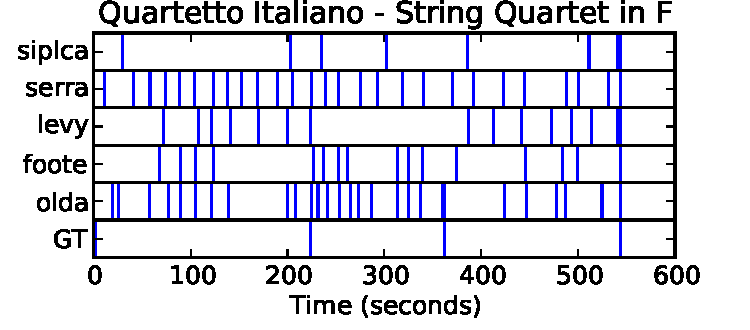
\includegraphics[width=0.45\textwidth, height=0.13\textheight]{plots/Quartetto-machine.pdf}
  \caption{Boundaries of one of the most difficult tracks to segment from a machine point of view.}
  \label{fig:quartetto}
\end{figure}%

\begin{figure}
  \centering
  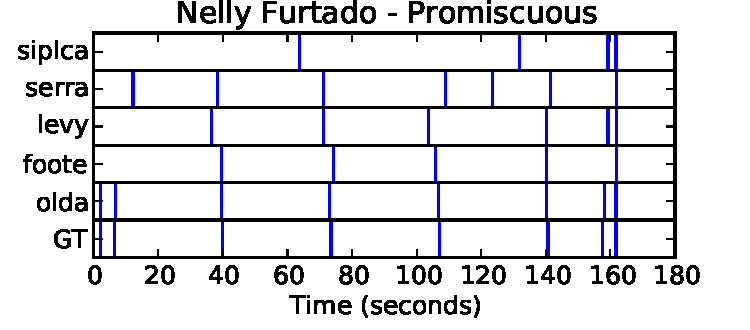
\includegraphics[width=0.45\textwidth, height=0.13\textheight]{plots/Promiscuous-machine.pdf}
  \caption{Boundaries of one of the tracks that machines find easiest to segment.}
  \label{fig:promiscuous}
\end{figure}%

Now that we can easily rank the tracks of the \textbf{BIG} dataset based on the MGP of the five selected algorithms we can start investigating why some of these pieces are so difficult to segment, at least from a machine perspective. 
One of the first ideas, that has been investigated before for the tasks of beat tracking \cite{Grosche2010} and chord recognition \cite{Ni2013}, is the problem of subjectivity.
%After listening to various hard tracks, we hypothesize that subjectivity might play a strong role in the detection of music boundaries, and we see why this may be actually the case in the next section. 
%We try to simplify the problem by obtaining a small dataset where multiple humans can annotate its tracks.
We aim to address this problem by obtaining multiple human annotations for a smaller dataset.

\subsection{Small Dataset}

Using the MGP, we create a small dataset that we refer to as \textbf{SMA} by selecting the hardest 45 tracks and the easiest 5 from the \textbf{BIG} dataset that meet the following requirements: (i) they are no longer than 10 minutes long (we want to keep the experiment time as low as possible to facilitate the work of the annotators and investigate a larger subset of tracks), and (ii) they are actual music pieces (in SALAMI we can find some tracks that are only speech fragments).

We filtered 6 tracks that agreed with one of these two principles in the hardest 45 (2 tracks were over 10 minutes and 4 tracks were only speech). 
Moreover, the average length for each song for the entire dataset is 244.1 seconds, whereas the average track length for the 45 hardest tracks selected (once we filtered the ones that met the defined criteria) is 348.5 seconds, which suggests a relation between difficulty and track length.
The 45 hardest tracks are composed by 8 tracks from the Cerulean dataset, 32 from the SALAMI dataset, and 5 from the Isophonics set.
It is interesting to note that no Epiphyte track was selected as difficult, even when almost half of the tracks in the \textbf{BIG} dataset are from the Epiphyte subset.
On the other hand, the easiest 5 tracks were composed of 3 Epiphyte tracks, 1 Isophonics, and 1 pop-rock SALAMI.
This suggests how the metric MGP is qualitatively working as expected, and therefore we are ready to obtain multiple annotations for this small dataset.

\subsection{Methodology}

We asked 5 music graduate students to identify the boundaries of the \textbf{SMA} dataset.
Even though it has been shown that the perception of boundaries in music does not depend on the musical background of the participants\cite{Bruderer2009}, these subjects had an average of 15 years of musical training.
We asked them to identify the boundaries, following the same guidelines as the ones used when collecting the data for SALAMI\cite{Smith2011}\footnote{URL to our guidelines are not displayed for submission}.
The participants used the Sonic Visualiser\cite{Cannam2006} in order to segment the 50 tracks, and they had to report at least one musical/acoustic tag for each one they found difficult to segment.
We start the analysis by taking a closer look to the reported tags.

\subsection{Qualitative Analysis of Difficulty}

We investigated all the reported tags and qualitatively clustered them into five main categories:

\begin{itemize}
  \item
    \textbf{Annotator}: This group contains tags that express a certain problem related with the annotator him/herself. 
    Examples: ``very ambiguous'', ``clueless''.

  \item
    \textbf{Audio Quality}: In this group the tags related with the physical nature of the recording are clustered. 
    Examples: ``noisy recording'', ``muffled''.

  \item
    \textbf{Form}: This group includes the tags related with the actual structure of the piece. Examples: ``long'', ``repetitive'', ``varied''.

  \item
    \textbf{Instrumentation}: Various tags that have to do with instrument peculiarities were also reported and included in this group. Examples: ``vocals only'', ``instrumental''.

  \item
    \textbf{Style}: The final group is the one related with the music genre of the piece, which includes, among other qualities, the speed and the homogeneity of the track. Examples: ``fast'', ``jazz''.
\end{itemize}

In Figure \ref{fig:difficult-tags-type} the frequency of each reported tag is shown, and it can be seen that two main clusters dominate the plot: style and form.
In terms of style, we hypothesize that there will be a strong bias depending on the preferred music genre of the subjects.
For example, there is considerable agreement on finding the jazz pieces difficult to segment, while all the subjects are classically trained.
On the other hand, the most reported tag of all the collection is the variability of a track, which falls in the form group (in red in the figure).
Other important tags inside this group are the extended duration of some pieces and the amount of repetition.

\begin{figure}
  \centering
  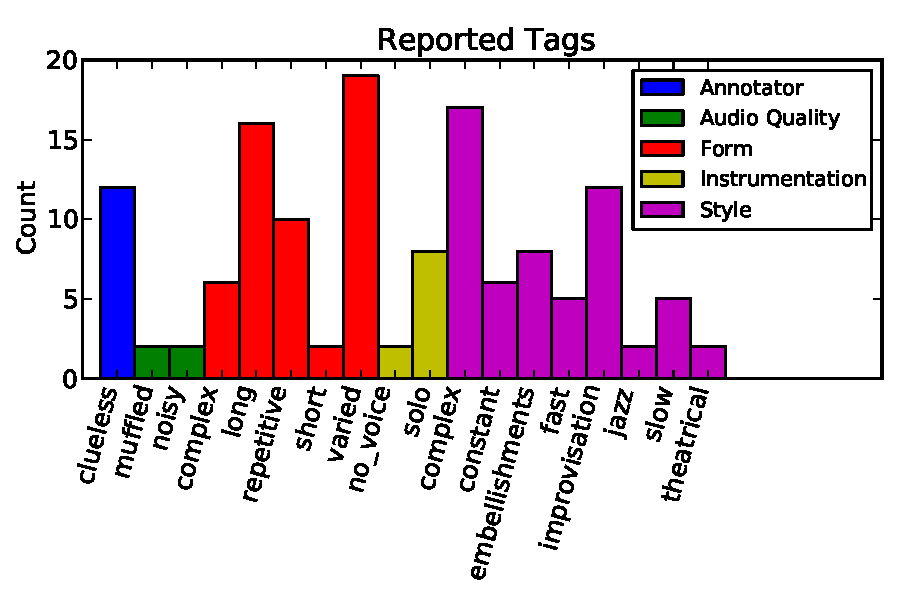
\includegraphics[width=0.47\textwidth]{plots/reported-tags.pdf}
  \caption{Number of reported tags for each of the qualitatively selected clusters.}
  \label{fig:difficult-tags-type}
\end{figure}%

Now that we have a better idea of the main qualities that make some tracks difficult to segment from a human perspective we aim to explore the actual boundaries reported by the subjects to test the amount of agreement among them, in order to apprehend a deeper understanding of the difficulties of this task.

\section{Quantitative Explorations}

%\subsection{Tags Agreement}

%Since tags were only submitted if humans found a specific track difficult to segment, we can easily check how uniformly humans reported tags for all the tracks of the \textbf{SMA} dataset.
%This would help us understand two main properties of the human data: (i) the degree of consistency when agreeing whether a track is difficult or not, and (ii) whether this agreement coordinates with the difficulty of segmenting tracks from a machine point of view.
%Note that we are not analyzing the new annotated boundaries yet, but only the reported subjective \textit{feeling} of degree of difficulty for all the given tracks.

%In Figure \ref{fig:human-difficulty} we see how many annotators reported at least one tag for each track in the \textbf{SMA} dataset.
%At a first glance we already see how the number of annotators reporting tags is almost uniformly distributed across the dataset, illustrating the lack of agreement. 
%The five tracks considered easy from a machine perspective are marked with a green rectangle, and based on where they are located in the plot we can see that tracks that machines found easy, humans generally find easy too.
%The two easy tracks from a machine perspective that contain one tag each are fairly short (a few seconds under a minute), and the reported tag, which is the same for both tracks, is precisely this: ``too short''.
%We will go back to these tracks when performing the analysis of the boundary annotations.

%TODO: Use Eric Figure to comment on this, and remember to talk about the control group.

%%\begin{figure}
  %%\centering
  %%\includegraphics[width=0.47\textwidth]{plots/human-difficulty.pdf}
  %%\caption{TODO}
  %%\label{fig:human-difficulty}
%%\end{figure}%

%%This may seem counterintuitive, since the longer the piece the harder it might seem to be segmented, but nevertheless only one subject reported difficulty when the track is too short, so it is not consistent with the rest of the subjects.


%We have seen that subjectivity might play an important role when evaluating music boundaries, at least from the qualitative perception of subjects.
%Now we will analyze the actual boundaries that subjects annotated to evaluate the degree of disagreement from a more objective data.

%Now we looked at the surface, now we're gonna look at this more closely.

\subsection{Analysis of the Multiple Human Boundaries}

In order to quantify the level of agreement between human annotations, we use the Mean Mutual Agreement (MMA) \cite{Holzapfel2012}.
Instead of comparing all the annotations against one ground truth (as we did in Section \ref{sub:hard-easy} using the MGP), we compare all the annotations with each other, since we might consider that now we have \textit{multiple ground truths}, given that all of these annotations, including the initial one, are done by humans.
In our case, the MMA does 15 comparisons ($N(N-1)/2$, where $N=6$ human annotations) using the hit rate measure as we did in the previous section.

The amount of agreement is depicted in Figure \ref{fig:human-agreement} where it becomes apparent that our annotators never agree with each other on this dataset more than at 65\% of the hit rate measure.
Moreover, the plot shows how these annotations tend to be ranked differently depending on what annotator they are being compared against.
This fact encourages us to explore the behavior of the algorithms when using different annotations in order to test the notion of ground truth for boundary detection.

\begin{figure}
  \centering
  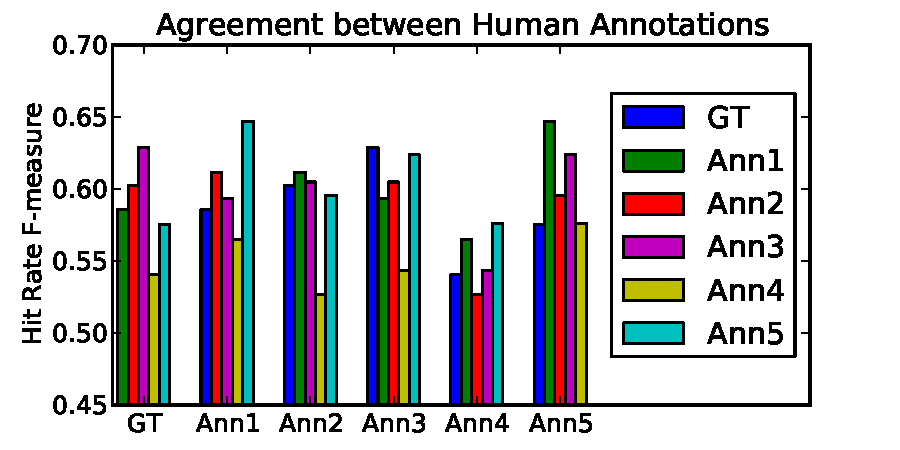
\includegraphics[width=0.47\textwidth]{plots/human-agreement.pdf}
  \caption{Boundary agreement among annotators.}
  \label{fig:human-agreement}
\end{figure}%

% TODO?:
%explore what multiple human perspectives can tell you about a consistently bad datapoint

\subsection{Using Multiple Annotations as Ground-truth}

We run our five different algorithms implemented in MSAF in the \textbf{SMA} dataset, and evaluate them against every human annotation available.
In Figure \ref{fig:annotatorsAsGT} we can see the scores for all the algorithms and annotations.

\begin{figure}
  \centering
  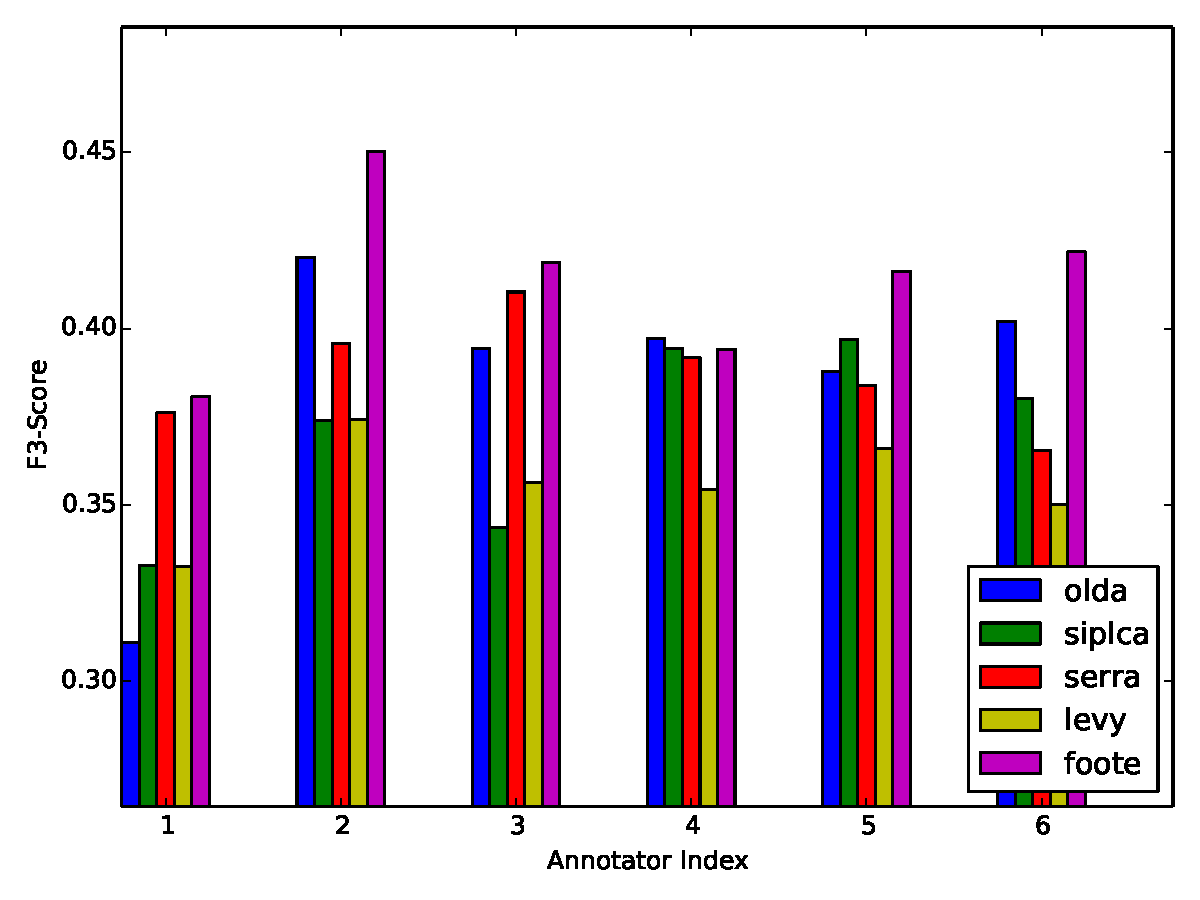
\includegraphics[width=0.47\textwidth]{plots/AnnotatorsAsGT.pdf}
  \caption{Algorithm scores for different human annotations as ground truth.}
  \label{fig:annotatorsAsGT}
\end{figure}%

In the figure we can see how the ranking of the algorithms changes depending on what annotation is used as ground truth.
We use the ranking stability measure in order to quantize this amount of variation, and show the results in table \ref{tab:stability-multipleGT}.
TODO: Table!
This illustrates that the notion of ground truth can be remarkably weak for boundary estimation, which becomes a serious problem when evaluating automatic approaches.

\begin{table}[h]
  \center
  \begin{tabular}{|c|c|}
    \hline
    Reference & Stability \\
    \hline
    GT      & TODO \\
    Ann1    & TODO \\
    Ann2    & TODO \\
    Ann3    & TODO \\
    Ann4    & TODO \\
    Ann5    & TODO \\
    \hline
  \end{tabular}
  \caption{Stability score for all the different annotators in the \textbf{SMA} dataset.}
  \label{tab:stability-multipleGT}
\end{table}


In order to approach this problem, we aim to use multiple annotations as a weighted single ground truth in order to produce more stable results.

\subsection{Weighted Boundaries}

We merge all the annotated boundaries for the \textbf{SMA} dataset by quantizing them into 1 second windows and then averaging them.
We normalize all the weighted boundaries such that the maximum weight is 1 for all the tracks in the dataset.
An example of this aggregation can be seen in Figure \ref{fig:merging-bounds}.

\begin{figure}
  \centering
  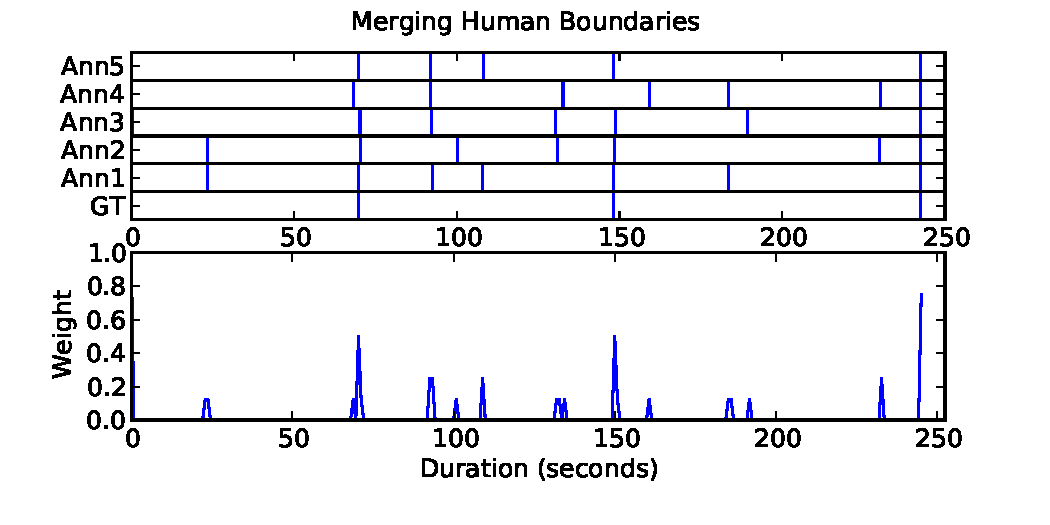
\includegraphics[width=0.47\textwidth]{plots/merging-bounds.pdf}
  \caption{Set of boundaries available on top for a given track (``You Never Give Me Your Money'', by The Beatles), and the weighted merged boundaries on the bottom.}
  \label{fig:merging-bounds}
\end{figure}

In order to evaluate these weighted boundaries we need to modify the actual hit rate method described in \ref{subsec:hitrate}.
Assuming we have a reference (or ground truth) of $N_r$ boundaries with associated weights $\textbf{w}_r = \{w_1, \ldots, w_{N_r}\}$, and an estimation of $N_e$ boundaries, we can compute the weighted hits $H$, composed of $N$ elements, as follows:

\begin{equation}
  H = h_1 w_{k_1} + \ldots + h_N w_{k_N}, \mbox{s.t.} w_i \in \textbf{w}_r
\end{equation}

where the indices $k_j$ correspond to those boundaries in the reference for which a hit has been found.
In this case, as in the standard evaluation, a hit is found when an estimated boundary is within 3 seconds from the closest reference one.

Once we have the weighted $H$ computed, we obtain the precision and the recall values by normalizing using the sum of the weights of the estimation and reference, respectively:

\begin{equation}
  P = \frac{H}{\sum \textbf{w}_e} , R = \frac{H}{\sum \textbf{w}_r}
\end{equation}

Since we only have $\textbf{w}_r$ (i.e. the implemented algorithms in MSAF do not output weighted estimations), we use the weights in $\textbf{w}_r$ to approximate $\textbf{w}_e$ as follows:
%when the estimated boundaries fall into a reference one, and the average across the reference weights for the rest of the estimated weights.

\begin{equation}
  \sum \textbf{w}_e = \sum_{j = 1}^{N} w_{k_j} + M \mu_{\textbf{w}_r}
\end{equation}

where $M$ is the number of estimated boundaries that are not considered hits.
The F-measure between the precision and the recall is computed as usual (see equation \ref{eq:fmeasure}).


%How subjective? Quite, for this particular subset. Name chords as a point of comparison, but realize that we cannot justify global subjectivity (i.e. boundary estimation can be subjective. not always, but certainly here). ≈75%, vs 90% for chords


%Evidence A: Ya, we can look at ??? (x) versus MMA of annotators (y) as a scatter plot, showing that there’s a spectrum to this subjectivity (insanity).

%Evidence B: Annotator Tags

%ScatPlot: \# of tags vs MMA

\subsection{Results of the Weighted Boundaries}

TODO: Eric: Talk about the stability depending on the annotator used. See how it is much more stable when we aggregate them.

Well, if you average multiple reference annotations, the rank order stability metric is more consistent (hopefully)

\section{Discussion and future perspectives}

Find a way to assess what tracks warrant multiple perspectives.

\section{Conclusions}

TODO.

\section{TODO}

Section2:
- stability rank

Section 3:
- ``data set sorting''
- Getting annotations

Section 4:
- Analysis of tags
- Gray out the tags figure.
- Talk control set (at least mention it)


Conclusion:
- How annotations should be done in the future


%\section{Boundaries Evaluation Metrics}\label{sec:evalmetrics}

%The boundaries of a given track are usually evaluated using the hit rate metric.
%In this section we review this evaluation and explore other metrics that might help addressing our goals.
%We refer the human annotated boundaries as \emph{reference}, and the ones identified by an algorithm as \emph{estimated}.

%\subsection{Hit Rate}\label{subsec:hitrate}

%The hit rate for boundaries evaluation is the most common and established metric for this task and it is traditionally used with a specific time window of 3 and/or 0.5 seconds\cite{Ong2005}. 

%This metric considers an estimated boundary as \emph{correct} (a hit) if it falls under the specified time window centered at its corresponding reference boundary.
%These hits are then used to compute three scores: the Precision ($P$, number of hits over the number of estimated boundaries), the Recall ($R$, number of hits over the number of reference boundaries), and the F-measure (harmonic mean between Precision and Recall), which is computed as follows:

%\begin{equation}
  %F = 2 \frac{P R}{P + R}
%\end{equation}

%\subsection{Median Deviations}

%This metric involves the computation of two median deviations: \emph{median reference to estimation} ($\sigma_{R2E}$) is the median in seconds from the reference boundaries to their nearest estimated ones, and the \emph{median estimation to reference} ($\sigma_{E2R}$) is analogous but swapping reference boundaries by estimated ones\cite{Pampalk}.
%Median deviations are not commonly reported in publications of boundary algorithms since the hit rate tends to be more reliable (note that, unlike the F-measure of the hit rate, these median deviations are not normalized and not compacted in a single score).
%However, they are, along with the hit rate, the only metrics included in MIREX to evaluate this task.

%\subsection{Information Gain}

%One of the most reliable metrics for beat tracking is the information gain\cite{Davies2009}. 
%This score has successfully been used to identify hard tracks (in terms of beat tracking) from a machine point of view from a large dataset without reference annotations\cite{Holzapfel2012}.
%This motivates us to explore its behavior when used for the task of boundary identification.

%The idea behind this metric is to treat the error between the reference and the estimation as a probability distribution.
%Typically, an error histogram of $K$ bins is used to capture these errors within a certain time range.
%The information gain $D$ can be seen as the inverse of the entropy of the probability distribution defined by the error histogram $p(z)$. Formally:

%\begin{equation}
  %D = \log_2(K) - H(p(z))
%\end{equation}

%If $p(z_k)$ is the probability mass of the bin $k$ of the error histogram, then $H(\cdot)$, which is the entropy function, can be defined as follows:

%\begin{equation}
  %H(p(z)) = \sum_{k=1}^K p(z_k) \log_2 \left( \frac{1}{p(z_k)} \right)
%\end{equation}

%Therefore we obtain a high $D$ if the error distribution is a prominent peak in the histogram (i.e. the error does not vary), whereas $D$ is low, close to 0, if the histogram is uniform (i.e. the error has a high degree of variation and the entropy is high).
%$D$ is bounded between 0 and $\log_2(K)$.
%We normalize this score by dividing it by $\log_2(K)$.

%Typically, in the task of beat tracking, histograms of $K=41$ bins are used within the range of $\pm0.5$ seconds.
%In our case, we use $K=250$ and an unrestricted time range in order to capture the higher errors that manifest in the boundary identification task compared to beat tracking.

%\subsection{Trimming First and Last Boundaries}

%The presented metrics treat all the boundaries of a given track equally. 
%However, we can argue that the first and last boundaries are trivial to be retrieved (the first boundary should always be placed in time 0, and the last one in the time defined by the duration of the track). 
%This topic was discussed in the music segmentation breaking session of last ISMIR edition\cite{Nieto2013}, and in a recent work by McFee only the trimmed scores are presented\cite{McFee2014}. 
%In this work we only present the trimmed version of the scores.

%\section{Machines Identifying Boundaries}\label{sec:eval_desc}

%Three different approaches have been established when classifying music boundaries: novelty, homogeneity, and repetition\cite{Paulus2010}. 
%Novelty-based approaches identify boundaries when there is a sudden change in some of the audio features (e.g. harmony, timbre).
%Homogeneity algorithms analyze blocks of audio and extract segment boundaries based on the consistency of these blocks, again based on one or more audio features.
%Finally, repetition-based methods aim to discover multiple occurrences of music patterns across the piece in order to identify the musical boundaries.

%In this work we aim to compare various automatic approaches in order to have a good understanding of the capability of machines when segmenting music.
%We select various segmentation algorithms and put them together in a Music Structural Analysis Framework (MSAF) to facilitate their execution, evaluation and analysis of results.

%\subsection{Music Structure Analysis Framework}

%A framework to compare various music segmentation algorithms, sharing their features and their evaluations, can be one of the most effective methodologies in order to explore and understand multiple algorithm behaviors.

%\subsubsection{Audio Features}

%To start with, we compute beat-synchronous audio features using Essentia\cite{Bogdanov2013}.
%The harmonic features are Harmonic Pitch Class Profiles (HPCP) and the timbral features are Mel-Frequency Cepstral Coefficients (MFCC), both features computed using Essentia's default parameters.
%The beats are detected using the multi-feature Essentia's beat tracker, and synchronized with the audio features using Ellis' method\cite{Ellis2007}.

%\subsubsection{Algorithm Selection}

%Two principles were applied when selecting the five algorithms to be used in this work: (i) The three different types of methodologies to extract boundaries should be represented, and (ii) the reported results of these methods should be competitive when compared with the state of the art.
%Note that this aims to emulate the behavior of having multiple human annotators segmenting the same tracks: not all of them will focus on the same type of boundaries (repetitive, homogeneous, novel), but we hope that all of them manage to retrieve fairly good quality boundaries in the end.

%Based on the previous principles, we select the following algorithms:

%\begin{itemize}
  %\item
    %\textbf{Foote}: One of the first music segmentation algorithms proposed, yet highly efficient and with good reported results\cite{Foote1999}. It is a novelty-based method that uses a Gaussian kernel across the diagonal of a self similarity matrix to identify sudden changes in the audio features.
  %\item
    %\textbf{Levy}: This approach uses Hidden Markov Model and constrained clustering to identify boundaries following a homogeneity-based principle\cite{Levy2008}.
  %\item
    %\textbf{Serr\`a}: This method defines the structural features, a set of features that combine both repeated and homogeneous boundaries. Once used to compute a novelty curve to extract the boundaries, this method combines the three different approaches to music segmentation, and reports some of the best scores for this task\cite{Serra2013}.
  %\item
    %\textbf{SI-PLCA}: Shift-Invariance Probabilistic Latent Component Analysis is an algorithm that uses a probabilistic variant of Non-negative Matrix Factorization in order to identify harmonic patterns with allowed key transpositions and time-shifted segments\cite{Weiss2011}. It can be seen as a repetition plus homogeneity-based approach.
  %\item 
    %\textbf{OLDA}: Ordinal Linear Discriminative Analysis uses the structural features defined in \cite{Serra2013} and applies a trained machine learning method (OLDA) to reduce their dimensionality and learn the most important set of features\cite{McFee2014}. This method obtains better results than Serr\`a's when using the hit rate at 0.5 seconds, and can be seen as an algorithm that also uses the three different principles of music segmentation.
%\end{itemize}

%\subsubsection{MSAF Performance}\label{subsub:performance}

%We use the Isophonics Beatles dataset\footnote{http://isophonics.net/content/reference-annotations-beatles} in order to show the performance of these five algorithms implemented in MSAF.
%This dataset is composed by the 180 tracks published by The Beatles and it is commonly used to evaluate music segmentation methods using the F-measure of the hit rate described in section \ref{subsec:hitrate} with a 3 seconds window, without trimming the first and last boundary.
%%Some of these algorithms only accept harmonic features (e.g. SI-PLCA), and others are designed to accept a mixture of them (e.g. OLDA).

%In Table \ref{tab:machine-algo-performance} we show the performance obtained in MSAF for each algorithm, including the type of features used.
%Note that we are reporting the trimmed version of the results (i.e. we do not compare the first and last boundaries), therefore these numbers are much lower than the ones reported in their original publications.
%However, if we were to compare our non-trimmed results (not shown in the table) with the reported results, we would find a small decrease in performance for some algorithms.
%We hypothesize that this arises from using slightly different parameters when computing the audio features, and/or by employing beat-synchronous features instead of standard frame-wise features.
%Moreover, there is variation between the scores, especially when comparing the F$_{0.5}$ scores across algorithms, but we believe it is important to maintain a good representation of all boundary types to better capture the behavior of the machines (e.g. Levy's method is, to the best of our knowledge, the best homogeneous-based segmentation algorithm, but its scores, in the Isophonics Beatles, are not as good as the algorithms that aim to identify boundaries based on novelty only).

%\begin{table}
 %\begin{center}
   %\begin{tabular}{|l|c|c|c|}
  %\hline
  %Algorithm & F$_3$ & F$_{0.5}$ & Feature\\
  %\hline
  %Foote     & 39.35 & 16.80 & MFCC\\
  %Levy      & 31.69 & 5.25 & MFCC\\
  %Serr\`a   & 58.18 & 16.32 & HPCP\\
  %SI-PLCA   & 26.98 & 5.54 & HPCP\\
  %OLDA      & 48.9 & 24.03 & Mix\\
  %\hline
 %\end{tabular}
%\end{center}
 %\caption{Performance of the MSAF in the Isophonics Beatles Dataset with the trimmed boundaries.}
 %\label{tab:machine-algo-performance}
%\end{table}

%Levy, OLDA and SI-PLCA implementations are available on-line as open source projects written by their first authors.
%Foote and Serr\`a methods were implemented from scratch specifically for this work.
%MSAF is an open-source project, where anyone can contribute with their segmentation algorithms\footnote{URL not displayed for revision process.}.

%\subsection{Big Dataset}\label{sub:dataset}

%In order to evaluate the algorithms in MSAF, we collected a large human annotated dataset of 2156 tracks that we refer to as \textbf{BIG} and is composed of four different datasets: Isophonics, SALAMI, Cerulean, and Epiphyte.

%\begin{itemize}
  %\item
    %\textbf{Isophonics}\footnote{http://isophonics.net/datasets}: This is the most common human-annotated dataset to analyze segmentation algorithms. 
    %It is composed of 300 tracks, including the 180 of The Beatles (discussed in \ref{subsub:performance}), of pop rock music by Queen, Michael Jackson, and others.

  %\item
    %\textbf{SALAMI}\cite{Smith2011}: The largest dataset with human-annotations for music segmentation published to date. 
    %It is composed of more than 700 tracks, with music types including classic, folk, world music, jazz, blues, and rock.
    %Some of these music genres can be particularly challenging to segment, both for machines and humans, as we will see in Section. %\ref{section:m-vs-h}.

  %\item
    %\textbf{Cerulean}: This dataset is a private annotation from a company that would like to remain anonymous.
    %It is composed by 102 particularly challenging tracks, including progressive rock, death metal, or classical music.

  %\item
    %\textbf{Epiphyte}: This is another private dataset from yet another anonymous company.
    %In this case over 1000 tracks were human-annotated, most of them being short pop rock and electronic songs.
    %The intuition is that these should be fairly easy tracks to segment, due to their simple musical structures.

%\end{itemize}

%\subsection{Metrics Comparison}

%We want to identify the tracks that machines find most difficult to segment.
%In order to do so, we need to use a specific metric, and sort the tracks based on this score.
%However, as we saw in Section \ref{sec:evalmetrics}, there are multiple metrics for boundary evaluation, so we first need to identify which one to use for sorting the tracks.

%We use the Mean Mutual Agreement (MMA) and Mean Performance Ground-truth (MGP) approach as in \cite{Holzapfel2012}.
%The MMA is the average of all the evaluations between algorithms (i.e. without using any human-annotated dataset).
%In our case, there are 10 comparisons ($N(N-1)/2$, where $N=5$ segmentation algorithms) for each one of the metrics.
%The MGP is the average performance of the 5 algorithms when compared with the human annotations.
%By comparing the MMA with the MGP we can tell how well a specific metric behaves in order to choose the best for our purposes.
%A histogram for each metric is computed by sorting the MMA results and placing their corresponding MGP scores in a 10 bin histogram to easily visualize how well the metric responds in all the different ranges of the score.

%In Figure \ref{fig:machine-eval-trim} we can see the histograms of the different metrics, sorted by their MMA value.
%As opposed to\cite{Holzapfel2012}, where beat trackers tend to agree most of the time, boundary algorithms usually perform far from perfectly.
%Therefore, it is a hard task to tell whether a given track is difficult to annotate solely by analyzing the MMA of a specific score.
%We can see that the median deviations (MMA$_{\sigma_{R2E}}$ and MMA$_{\sigma_{E2R}}$, which are normalized using the maximum deviation time) are mostly contained in a short range of the histogram, especially MMA$_{\sigma_{E2R}}$.
%The information gain (MMA$_D$) is contained in a single histogram bin most of the time, making it difficult to predict hard tracks from just the MMA$_D$, since even in the worst MMA$_D$ track range, we find scores in their respective MPG$_D$ that fall in bins where only the easy tracks should be placed.
%Finally, the MMA$_{F05}$ is too much spread across the histogram bins, with almost a flat spread curve.
%However, the MMA$_{F3}$ seems to be the only metric that ranges almost all the histogram bins from hardest to easiest with a relatively narrow curve.

%\begin{figure}
      %\centering
      %\begin{subfigure}[b]{0.25\textwidth}
              %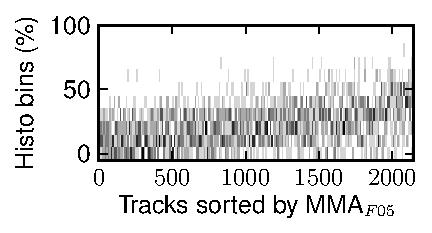
\includegraphics[width=\textwidth]{plots/histo-F05-trim.pdf}
              %%\caption{Histogram of F-measure 0.5}
              %\caption{}
              %\label{fig:histo-F05-trim}
      %\end{subfigure}%
      %~ 
      %\begin{subfigure}[b]{0.25\textwidth}
              %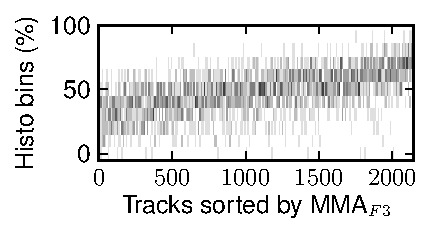
\includegraphics[width=\textwidth]{plots/histo-F3-trim.pdf}
              %\caption{}
              %\label{fig:histo-F3-trim}
      %\end{subfigure}%
       
      %\begin{subfigure}[b]{0.25\textwidth}
              %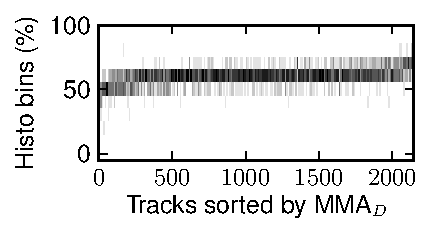
\includegraphics[width=\textwidth]{plots/histo-D-trim.pdf}
              %\caption{}
              %\label{fig:histo-D-trim}
      %\end{subfigure}%
      %~ 
      %\begin{subfigure}[b]{0.25\textwidth}
              %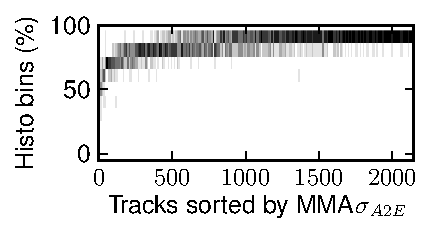
\includegraphics[width=\textwidth]{plots/histo-DevA2E-trim.pdf}
              %\caption{}
              %\label{fig:histo-DevA2E-trim}
      %\end{subfigure}%
       
      %\begin{subfigure}[b]{0.25\textwidth}
              %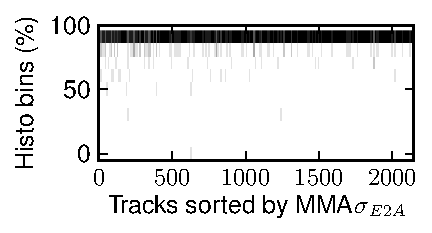
\includegraphics[width=\textwidth]{plots/histo-DevE2A-trim.pdf}
              %\caption{}
              %\label{fig:histo-DevE2A-trim}
      %\end{subfigure}%

      %\caption{MMA vs MGP histograms of the Machine-analyzed tracks.}\label{fig:machine-eval-trim}
%\end{figure}

%We argue that these metrics (or maybe the task itself) are still not able to predict hard and easy tracks from datasets without human-annotations, but the $F3$ metric qualitatively seems to behave the best of the ones tested here.
%Therefore, we will use this evaluation in order to find the hardest and easiest tracks on our human-annotated dataset.

%\subsection{Hardest and Easiest Tracks}\label{sub:hard-easy}

%We run our algorithms on our \textbf{BIG} dataset described in Section \ref{sub:dataset} and sort their tracks based on their MGP$_{F3}$ scores.
%Thus, we are able to know which are the tracks of our dataset that machines find easiest and hardest to segment by simply exploring the beginning or the end of the sorted list.

%In Figures \ref{fig:quartetto} and \ref{fig:promiscuous} we show examples of the boundaries of all the algorithms for a hard and an easy track, respectively, from a machine point of view.
%The difficult track is a classical piece (string quartet) over 9 minutes long, and we can see the little agreement among algorithms when comparing their extracted boundaries.
%The easy one is a popular dance song that is less than 3 minutes long, with a much higher degree of agreement.

%\begin{figure}
  %\centering
  %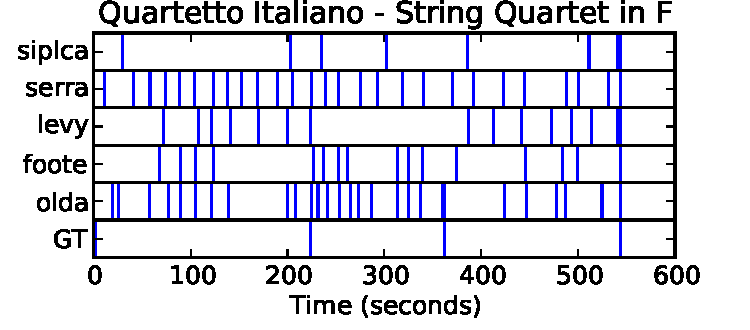
\includegraphics[width=0.45\textwidth, height=0.13\textheight]{plots/Quartetto-machine.pdf}
  %\caption{Boundaries of one of the most difficult tracks to segment from a machine point of view.}
  %\label{fig:quartetto}
%\end{figure}%

%\begin{figure}
  %\centering
  %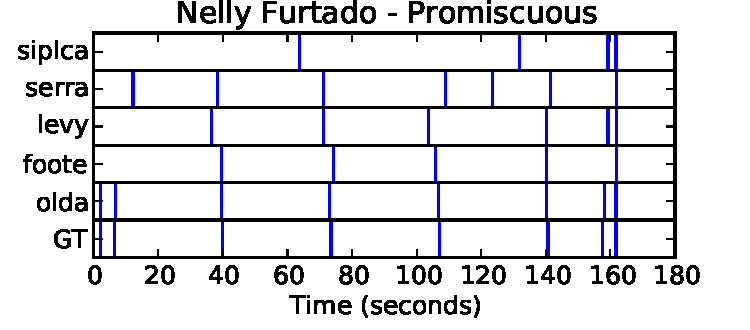
\includegraphics[width=0.45\textwidth, height=0.13\textheight]{plots/Promiscuous-machine.pdf}
  %\caption{Boundaries of one of the tracks that machines find easiest to segment.}
  %\label{fig:promiscuous}
%\end{figure}%

%The hardest tracks have a tendency of being longer in duration than the easier ones.
%We can see this behavior in Figure \ref{fig:machinesdur}, where we see the tracks sorted by MGP$_{F3}$, which indicates that duration can have an impact in music segmentation from a machine point of view.

%\begin{figure}
  %\centering
  %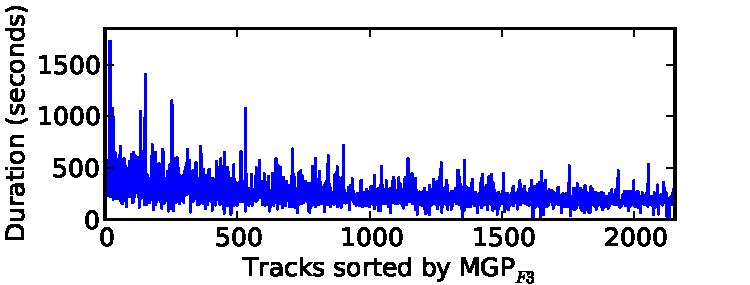
\includegraphics[width=0.45\textwidth, height=0.13\textheight]{plots/machines-duration.pdf}
  %\caption{Duration of all the tracks in the \textbf{BIG} dataset.}
  %\label{fig:machinesdur}
%\end{figure}%

%We can now proceed with a similar technique to identify the hardest and easiest tracks to segment from a human point of view.

%\section{Humans Identifying Boundaries}\label{sec:using_method}

%In this section we describe the process of segmenting music from a human perspective, and aim to identify the tracks that we, as humans, find hard (or easy) to segment. 
%To do so we create a smaller dataset that is used to run an experiment and then analyze the results using similar methods as described in the previous section.

%\subsection{Small Dataset}

%Using the technique described in Section \ref{sub:hard-easy}, we create a small dataset that we refer as \textbf{SMA} by selecting the hardest 45 tracks and the easiest 5 from the \textbf{BIG} dataset that meet the following requirements: (i) they are no longer than 10 minutes long, and (ii) they are actual music pieces (in SALAMI we can find some tracks that are only speech fragments).

%We filtered 6 tracks that agreed with one of these two principles in the hardest 45 (2 tracks were over 10 minutes and 4 tracks were only speech). 
%Moreover, the average length for each song for the entire dataset is 244.1 seconds, whereas the average track length for the 45 hardest tracks selected (once we filtered the ones that met the defined criteria) is 348.5 seconds.
%The 45 hardest tracks are composed by 8 tracks from the Cerulean dataset, 32 from the SALAMI dataset, and 5 from the Isophonics set.
%It is interesting to note that no Epiphyte track was selected as difficult, even when almost half of the tracks in the \textbf{BIG} dataset are from the Epiphyte subset.
%On the other hand, the easiest 5 tracks were composed of 4 Epiphyte tracks and 1 Isophonics.
%This shows how the metric MGP$_{F3}$ is qualitatively working as expected.


%\subsection{Experiment Setup}

%We asked 5 music graduate students to identify the boundaries of the \textbf{SMA} dataset.
%Even though it has been shown that the perception of boundaries in music does not depend on the musical background of the participants\cite{Bruderer2009}, these subjects had an average of 11 years of musical training.
%We asked the subjects to identify the boundaries, following very similar guidelines as the ones used when collecting the data for SALAMI\cite{Smith2011}\footnote{URL to our guidelines are not displayed for submission}.
%The participants used the Sonic Visualiser\cite{Cannam2006} in order to segment the 50 tracks, and for each one they found difficult to segment, they had to report at least one musical/acoustic tag.

%\subsection{Analysis of the Results}

%We first compute the MMA of the results of the humans and compare it with their MGP for each one of the metrics (see Figure \ref{fig:human-eval}).
%One would expect to find a strong agreement, since we are simply comparing a human annotation (the original ground-truth) with 5 other human-annotated results from the experiment.
%However, these plots show that the agreement is far from perfect, indicating the inherent complexity of the task, which tends to be highly subjective in multiple occasions.
%We also see that F$_3$ is still the metric that could better predict hard and easy tracks to segment, this time from a human point of view, even though it might be not good enough.
%Therefore, even if machines would obtain results similar to those obtained by humans, we would need other evaluations or datasets in order to automatically predict the difficulty of a given track.

%\begin{figure}
      %\centering
      %\begin{subfigure}[b]{0.25\textwidth}
              %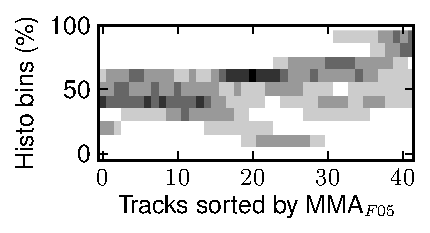
\includegraphics[width=\textwidth]{plots/histo-human-F05.pdf}
              %%\caption{Histogram of F-measure 0.5}
              %\caption{}
              %\label{fig:histo-human-F05}
      %\end{subfigure}%
      %~ 
      %\begin{subfigure}[b]{0.25\textwidth}
              %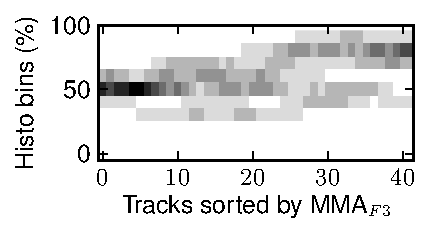
\includegraphics[width=\textwidth]{plots/histo-human-F3.pdf}
              %\caption{}
              %\label{fig:histo-human-F3}
      %\end{subfigure}%
       
      %\begin{subfigure}[b]{0.25\textwidth}
              %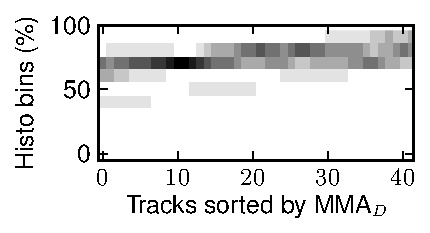
\includegraphics[width=\textwidth]{plots/histo-human-D.pdf}
              %\caption{}
              %\label{fig:histo-human-D}
      %\end{subfigure}%
      %~ 
      %\begin{subfigure}[b]{0.25\textwidth}
              %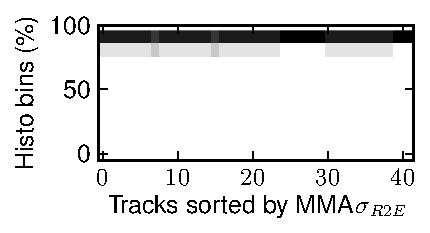
\includegraphics[width=\textwidth]{plots/histo-human-DevA2E.pdf}
              %\caption{}
              %\label{fig:histo-human-DevA2E}
      %\end{subfigure}%
       
      %\begin{subfigure}[b]{0.25\textwidth}
              %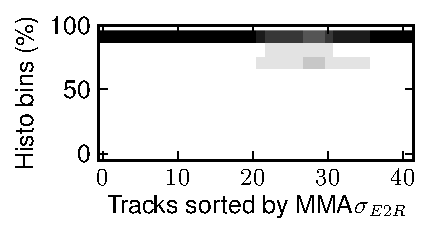
\includegraphics[width=\textwidth]{plots/histo-human-DevE2A.pdf}
              %\caption{}
              %\label{fig:histo-human-DevE2A}
      %\end{subfigure}%

      %\caption{MMA vs MGP histograms of the Human-analyzed tracks.}\label{fig:human-eval}
%\end{figure}

%After sorting the human results using the MGP$_{F3}$, we can easily examine the worst and best results from a human perspective.
%In Figures \ref{fig:starship-human} and \ref{fig:promiscuous-human} we show examples of the most difficult and easiest tracks, respectively, from a human perspective.
%In this case, one of the most difficult tracks is a 9 minute long progressive rock song by Yes.
%We see that the original annotator (marked as GT) over-segmented the track compared with the subjects of the experiment.
%However, there are some very prominent boundaries that all the annotators identified (e.g. in second 337 a sudden change in timbre and harmony occurs, changing from a complex part with all the instruments of the rock band to a clean guitar solo repeating a simple chord pattern).
%On the other hand, one of the easiest tracks to segment from a human perspective coincides with the one exemplified for machines (see Figure \ref{fig:promiscuous}).
%The mutual agreement of this track is quite high, especially for F$_3$, since there are a few boundaries that some subjects misplaced a few seconds before/after the original GT annotation.

%\begin{figure}
  %\centering
  %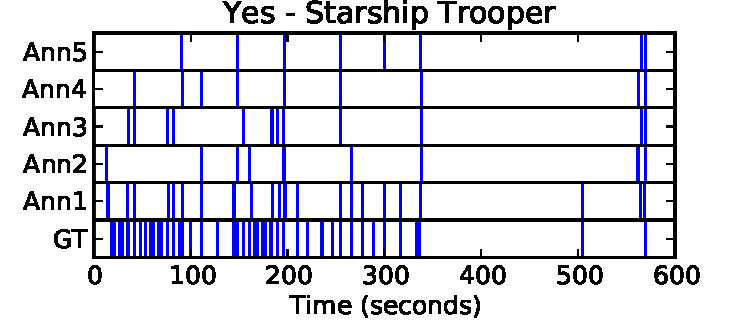
\includegraphics[width=0.45\textwidth, height=0.13\textheight]{plots/StarshipTrooper-human.pdf}
  %\caption{One of the most difficult tracks to segment from a human point of view.}
  %\label{fig:starship-human}
%\end{figure}%

%\begin{figure}
  %\centering
  %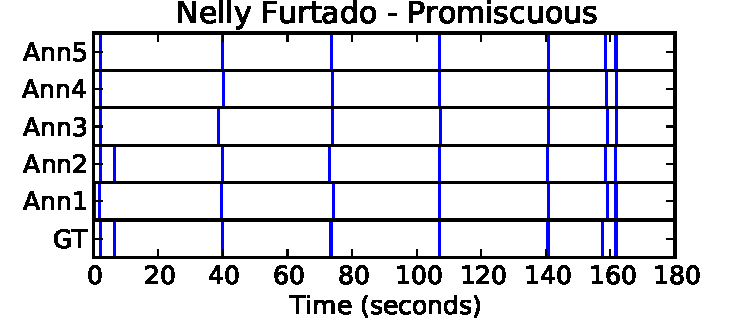
\includegraphics[width=0.45\textwidth, height=0.13\textheight]{plots/Promiscuous-human.pdf}
  %\caption{One of the tracks that humans find easiest to segment.}
  %\label{fig:promiscuous-human}
%\end{figure}%

%We investigate the influence of the duration of the tracks as we did for the machines.
%In this case, the duration does not seem to correlate much with the performance of the subjects, as shown in Figure \ref{fig:humansdur}.
%However, most of these tracks were over 5 minutes long, so we should have a broader dataset in order to formally conclude that duration is not an important factor for humans when identifying boundaries.

%\begin{figure}
  %\centering
  %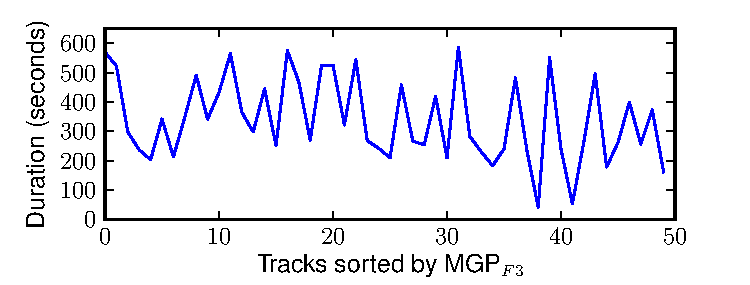
\includegraphics[width=0.45\textwidth, height=0.13\textheight]{plots/humans-duration.pdf}
  %\caption{Duration of all the tracks in the \textbf{SMA} dataset.}
  %\label{fig:humansdur}
%\end{figure}%

%When analyzing the answers from the subjects, in order to know what are the audio features that make it hard to segment the song we see that the longer tracks were the ones that humans found most difficult to segment from a subjective perspective.
%Another factor was the repetitiveness quality of the song: if the song is either too repetitive or too little repetitive makes it harder to segment for humans.
%The jazz improvisations were also reported as hard to segment, which might also have to do with the fact that some tracks were notoriously hard to segment because they were difficult to memorize.
%(TODO: Add histogram of tags?).

%\section{Machines vs Humans}\label{section:m-vs-h}

%In the histograms comparing the MMA and MGP of the machines and humans (Figures \ref{fig:machine-eval-trim} and \ref{fig:human-eval}) we see that humans tend to agree with the original ground truth much more than machines (note that for metrics F$_3$, F$_{0.5}$ and $D$ the energy in the histograms is located in much higher bins).
%This is interesting by itself, since it implies that there is still room for improvement in the boundary algorithms.

%One of our main goals is to identify those tracks that machines find difficult to segment while humans can do a good job about it.
%In order to do so, we compare the MGP$_{F3}$ between machines and humans for all the tracks in \textbf{SMA}, and plot the comparison in Figure \ref{fig:machines-vs-humans}.
%In this plot we can see two main clusters of tracks: the ones that machines find easy to segment (dots in the upper right corner), and the ones that have been identified as hard (dots on the left).
%Marked in the plot are the easy tracks for both machines and humans (red ellipse), the hard tracks for both as well (magenta square), and the hard and easy tracks for machines and humans respectively (green circle).

%\begin{figure}
  %\centering
  %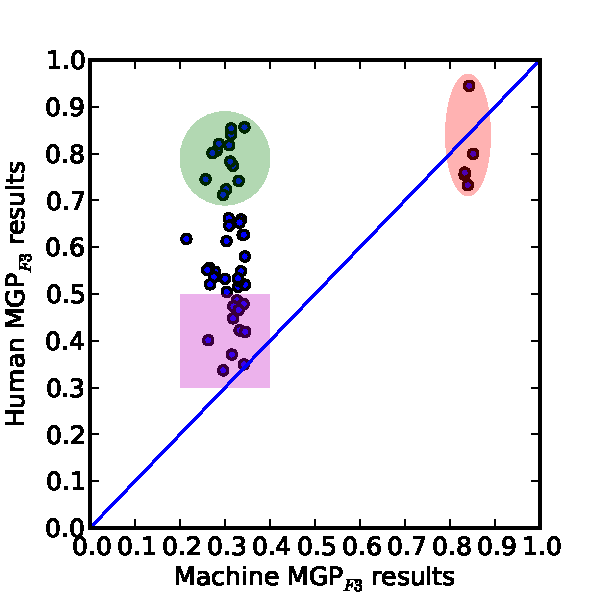
\includegraphics[width=0.45\textwidth, height=0.28\textheight]{plots/machines-vs-humans.pdf}
  %\caption{Comparison between the MGP$_{F3}$ of Machines and Humans.}
  %\label{fig:machines-vs-humans}
%\end{figure}%

%\subsection{Easy tracks for both}

%Marked with a red ellipse are the 5 tracks that were identified as easy by machines.
%We can see that humans agree with machines in this case, obtaining high scores as well.
%These tracks are mostly popular dance and rock songs with a simple structure and short duration.

%\subsection{Hard tracks for both}

%These tracks are marked with a magenta square, and they tend to be the longest ones in \textbf{SMA}.
%Humans apparently have a hard time segmenting these tracks, so we can not expect machines to do a better work in general.
%Therefore, we are not genuinely interested in this subset of tracks, since they can not help us improve the current state-of-the-art boundary algorithms.
%Examples of these tracks are Starship Trooper by Yes, or flamenco improvisations.

%\subsection{Machine Hard vs Human Easy}

%In this subset of tracks we might find relevant information in order to improve automatic algorithms to identify boundaries.
%We analyze the 12 tracks marked with a green circle, which are the ones that are easy to segment from a human point of view and hard from a machine perspective.

%To start with, 10 of these tracks contain either live performances or genres where the tempo slightly varies.
%This might make the beat tracker fail, which results in a worse performance for machines when using beat-synchronous features.
%Interestingly, 6 out 12 of these tracks are slightly out of tune.
%This makes the algorithms that rely solely on harmonic features like HPCP to fail, while humans do a good job about it.
%5 of these tracks are longer than 8 minutes, but in this case this does not seem to affect humans, since in all of these long tracks the parts were very differentiated (e.g. the jazz improvisation in SALAMI 444 has applauses in between solos, which clearly mark a boundary between its different segments).
%An interesting track is SALAMI 584, where a sax plays the popular melody of ``Over the Rainbow''.
%The rhythm of the sax is quite expressive, with high tempo variations, but the fact that it plays a very familiar melody makes it easy to segment from a human point of view.



%%SALAMI 546: Out of tune, expressive timing.
%%Cerulean Bob Dylan Like a Rolling Stone: Out of tune, live version, expressive timing.
%%Cerulean Bob Dylan Hurricane: Out of tune, live version, expressive timing.
%%Cerulean Leonard Bern: Classical, long, expressive timing.
%%SALAMI 584: Interesting jazz version of Over The Rainbow.
%%SALAMI 12: expressive timing, only voice, complex harmony
%%Isophonics Don't pass me by: Out of tune (violin)
%%SALAMI 1198: Long, jazz improvisations
%%SALAMI 1324: Out of tune, live recording, expressive timing
%%SALAMI 20: Blues improvisation, expressive timing
%%SALAMI 278: Classical music, expressive timing
%%SALAMI 444: JAzz improvisation, exprissive timing, long





%%\begin{table}
 %%\begin{center}
 %%\begin{tabular}{|l|l|}
  %%\hline
  %%String value & Numeric value \\
  %%\hline
  %%Hello ISMIR  & 2014 \\
  %%\hline
 %%\end{tabular}
%%\end{center}
 %%\caption{Table captions should be placed below the table.}
 %%\label{tab:example}
%%\end{table}

%%\begin{figure}
 %%\centerline{\framebox{
 %%\includegraphics[width=\columnwidth]{figure.png}}}
 %%\caption{Figure captions should be placed below the figure.}
 %%\label{fig:example}
%%\end{figure}

%\section{Experiment 1}

%\begin{table}
 %\begin{center}
   %\begin{tabular}{|l|c|c|c|c|c|}
  %\hline
  %Reference & F$_3$ & F$_{0.5}$ & $D$ & $\sigma_{R2E}$ & $\sigma_{E2R}$\\
  %\hline
  %GT          & 34.66 & 23.17 & 0.526 & 6.49 & 9.83 \\
  %Ann1        & \textbf{40.29} & 26.49 & 0.529 & 6.24 & 8.37 \\
  %Ann2        & 38.47 & 24.62 & 0.515 & 6.04 & \textbf{7.87} \\
  %Ann3        & 38.64 & 25.03 & 0.535 & 5.31 & 9.08 \\
  %Ann4        & 39.02 & \textbf{26.59} & \textbf{0.547} & 6.54 & 8.54 \\
  %Ann5        & 38.39 & 25.94 & 0.536 & \textbf{5.04} & 9.86 \\
  %\hline
 %\end{tabular}
%\end{center}
 %\caption{Performance of the MSAF in the Isophonics Beatles Dataset with the trimmed boundaries.}
 %\label{tab:experiment1}
%\end{table}

%\section{Experiment 3a}

%\begin{table}
 %\begin{center}
   %\begin{tabular}{|l|c|c|}
  %\hline
  %Reference & std(F$_3$) & std(F$_{0.5}$) \\
  %\hline
  %GT          & 15.74 & 12.02 \\
  %Ann1        & 15.06 & 12.41 \\
  %Ann2        & 15.10 & 11.70 \\
  %Ann3        & 15.20 & 11.38 \\
  %Ann4        & 15.45 & 12.56 \\
  %Ann5        & 15.25 & 11.84 \\
  %\hline
  %Merged      & 6.88 & 9.83 \\
  %\hline
 %\end{tabular}
%\end{center}
 %\caption{TODO}
 %\label{tab:experiment3a}
%\end{table}

%\section{Conclusions}

%TODO.

%Identified some audio properties that could improve the automatic segmentation algorithms.


%\begin{thebibliography}{citations}

%\bibitem {Author:00}
%E. Author:
%``The Title of the Conference Paper,''
%{\it Proceedings of the International Symposium
%on Music Information Retrieval}, pp.~000--111, 2000.

%\bibitem{Someone:10}
%A. Someone, B. Someone, and C. Someone:
%``The Title of the Journal Paper,''
%{\it Journal of New Music Research},
%Vol.~A, No.~B, pp.~111--222, 2010.

%\bibitem{Someone:04} X. Someone and Y. Someone: {\it Title of the Book},
    %Editorial Acme, Porto, 2012.

%\end{thebibliography}

%\small
\bibliography{references}

\end{document}
